\documentclass[ignorenonframetext]{beamer}

\usepackage{listings}

\usepackage{graphicx}
\usepackage{caption}
\usepackage{subcaption}
% \usepackage{subfig}
%\usepackage{floatrow}

%\usepackage{url}
% =========================================
% http://www.pletscher.org/writings/latex/beamerthemes.php
\usetheme{Berlin}   
%\usetheme{Frankfurt}
%\usetheme{Darmstadt}
%\usetheme{Boadilla}
%\usetheme{Madrid}  %%%%
%\usetheme{Pittsburgh}
%\usetheme{Rochester}
%\usetheme{Copenhagen}
%\usetheme{Warsaw}
%\usetheme{Singapore}
%\usetheme{Malmoe}
% =========================================
%\definecolor{bybg}{rgb}{1,1,1}
%\definecolor{bybg}{gray}{.8}  


%gets rid of bottom navigation bars
%\setbeamertemplate{footline}[page number]{}
\setbeamertemplate{footline}{}
%gets rid of navigation symbols
%\setbeamertemplate{navigation symbols}{}



% set the block-width
\addtobeamertemplate{block begin}{\setlength{\textwidth}{1.0\textwidth}}{}

\newenvironment<>{halfblock}[2][.5\textwidth]{%
  \setlength{\textwidth}{#1}
  \begin{actionenv}#3%
    \def\insertblocktitle{#2}%
    \par%
    \usebeamertemplate{block begin}}
  {\par%
    \usebeamertemplate{block end}%
  \end{actionenv}}


\definecolor{darkgreen}{rgb}{0,.6,0}

\lstset{
   language=C++,
   frame=shadowbox,
   basicstyle=\scriptsize\ttfamily,
%    keywordstyle=\bfseries\ttfamily\color{green},
   stringstyle=\color{black}\ttfamily,
   rulesepcolor=\color{gray},
   tabsize=2,
   %emphstyle=\color{blue}\texttt
   commentstyle=\color{blue}\ttfamily,
   %numbers=left,
   %numberstyle=\tiny,
   showstringspaces=false,
   literate={~} {$\sim$}{1},
   tagstyle=\ttfamily\footnotesize\color{blue},
   moredelim=[is][\color{red}]{!<}{>!},%,
   escapechar=|
%   linewidth=0.9\textwidth
   %moredelim=[is][\color{darkgreen}]{-}{-}   
%   stringstyle=\color{red}
}
%\definecolor{mytest}{\color{gray}}{0.9}
%\newcommand{\Hilight}{\makebox[0pt][l]{\color{BrickRed}\rule[-4pt]{0.65\linewidth}{14pt}}}
%\newcommand{\Hilight}{\makebox[0pt][l]{\color{cyan}\rule[-4pt]{1.0\linewidth}{14pt}}}


%\urlstyle{tt}
%\urldef{\iueweb}{\url}{http://www.iue.tuwien.ac.at}

% =========================================
\beamertemplatenavigationsymbolsempty
%\setbeamertemplate{footline}[frame number]
\setbeamercovered{transparent}
% =========================================

% =========================================
%\logo{\includegraphics[width=9.0cm]{pics/sky_iuecol.eps}}
%\logo{\includegraphics[width=9.0cm]{pics/sky_iuecol-rep.eps}}
\logo{\vspace{-0.3cm}\includegraphics[width=9.0cm]{pics/sky_iuecol.eps}}
%\pgfdeclareimage[height=1cm]{unilogo}{pics/TU_Signet_CMYK.eps}
%\usebackgroundtemplate{\includegraphics{pics/sky_iuecol.eps}}
% =========================================
\title{ViennaMesh\\A Highly Flexible Meshing Framework}

\author{\underline{Florian Rudolf}, Josef Weinbub, Karl Rupp,\\ and Siegfried Selberherr}
\date{}
\institute[FEMTEC - Las Vegas, USA - May, 2013]{}

\titlegraphic{
   \begin{figure}[!ht]
   \vspace{-1.0cm}
   \begin{minipage}{1.5cm}
      \begin{center} 
         \includegraphics[width=1.2cm]{pics/TU_Signet_CMYK.eps}
      \end{center}
   \end{minipage}
   \hfill
   \begin{minipage}{5.5cm}
      \begin{center}
      \scriptsize%\textsc{
      Institute for Microelectronics\\
      Technische Universit\"at Wien\\
      Vienna - Austria - Europe\\
      http:/$\negthinspace$/www.iue.tuwien.ac.at
      %}
      \end{center}
   \end{minipage}   
   \hfill   
   \begin{minipage}{1.5cm}
      \begin{center}
         
\includegraphics[width=1.4cm]{pics/logo_px500.ps}
      \end{center}      
   \end{minipage}
\end{figure}
}


\begin{document}





\frame{\titlepage}

% ==============================================================================
\frame{
   \frametitle{Table of Contents}
   \tableofcontents
}

% ==============================================================================
\section{Overview}
\subsection{}

\begin{frame}[fragile]%[<+->]
  \frametitle{What Is ViennaMesh?}
  
  \begin{block}{Open source C++ meshing framework}
    \begin{itemize} \footnotesize
      \item LGPL
    \end{itemize}
  \end{block}

  \begin{block}{Based on a highly flexible data structure}
    \begin{itemize} \itemsep0pt \footnotesize
      \item Focus on abstract topology and orthogonality
    \end{itemize}
  \end{block}
  
  \begin{block}{Abstract concepts enable uniform interfaces}
    \begin{itemize} \itemsep0pt \footnotesize
      \item Generic programming
    \end{itemize}
  \end{block}
  
\end{frame}



\begin{frame}[fragile]%[<+->]
  \frametitle{Problems Addressed by ViennaMesh}
  
  \begin{block}{Simultaneous use of different meshing algorithms/libraries}
    \begin{itemize} \itemsep0pt \footnotesize
      \item Challenging due to incompatible data structures and interfaces
    \end{itemize}
  \end{block}
  
  \begin{block}{Extensibility}
    \begin{itemize} \itemsep0pt \footnotesize
      \item Most libraries are hard to extend
    \end{itemize}
  \end{block}
  
  \begin{block}{Reusability}
    \begin{itemize} \itemsep0pt \footnotesize
      \item Code written against a library can hardly be reused with another library
    \end{itemize}
  \end{block}
  
  \begin{block}{Flexibility}
    \begin{itemize} \itemsep0pt \footnotesize
      \item Data structure of libraries is often static and inflexible
    \end{itemize}
  \end{block}
  
\end{frame}



\begin{frame}[fragile]%[<+->]
  \frametitle{Framework Details}

  \begin{block}{C++ library}
    \begin{itemize} \itemsep0pt \footnotesize
      \item Data structure and core functionality header-only
      \item C++11 support
      \item Cmake support
    \end{itemize}
  \end{block}
  
  \begin{block}{Interfaces to proven libraries}
    \begin{itemize} \itemsep0pt \footnotesize
      \item Meshing: Netgen, CGAL, VERDICT
      \item Statistics: Boost.Accumulators
      \item More to come: Tetgen, Triangle, Mesquite, Metis, ...
    \end{itemize}
  \end{block}
  
\end{frame}



\begin{frame}[fragile]%[<+->]
  \frametitle{Framework Overview}

    \begin{figure}
        \centering
        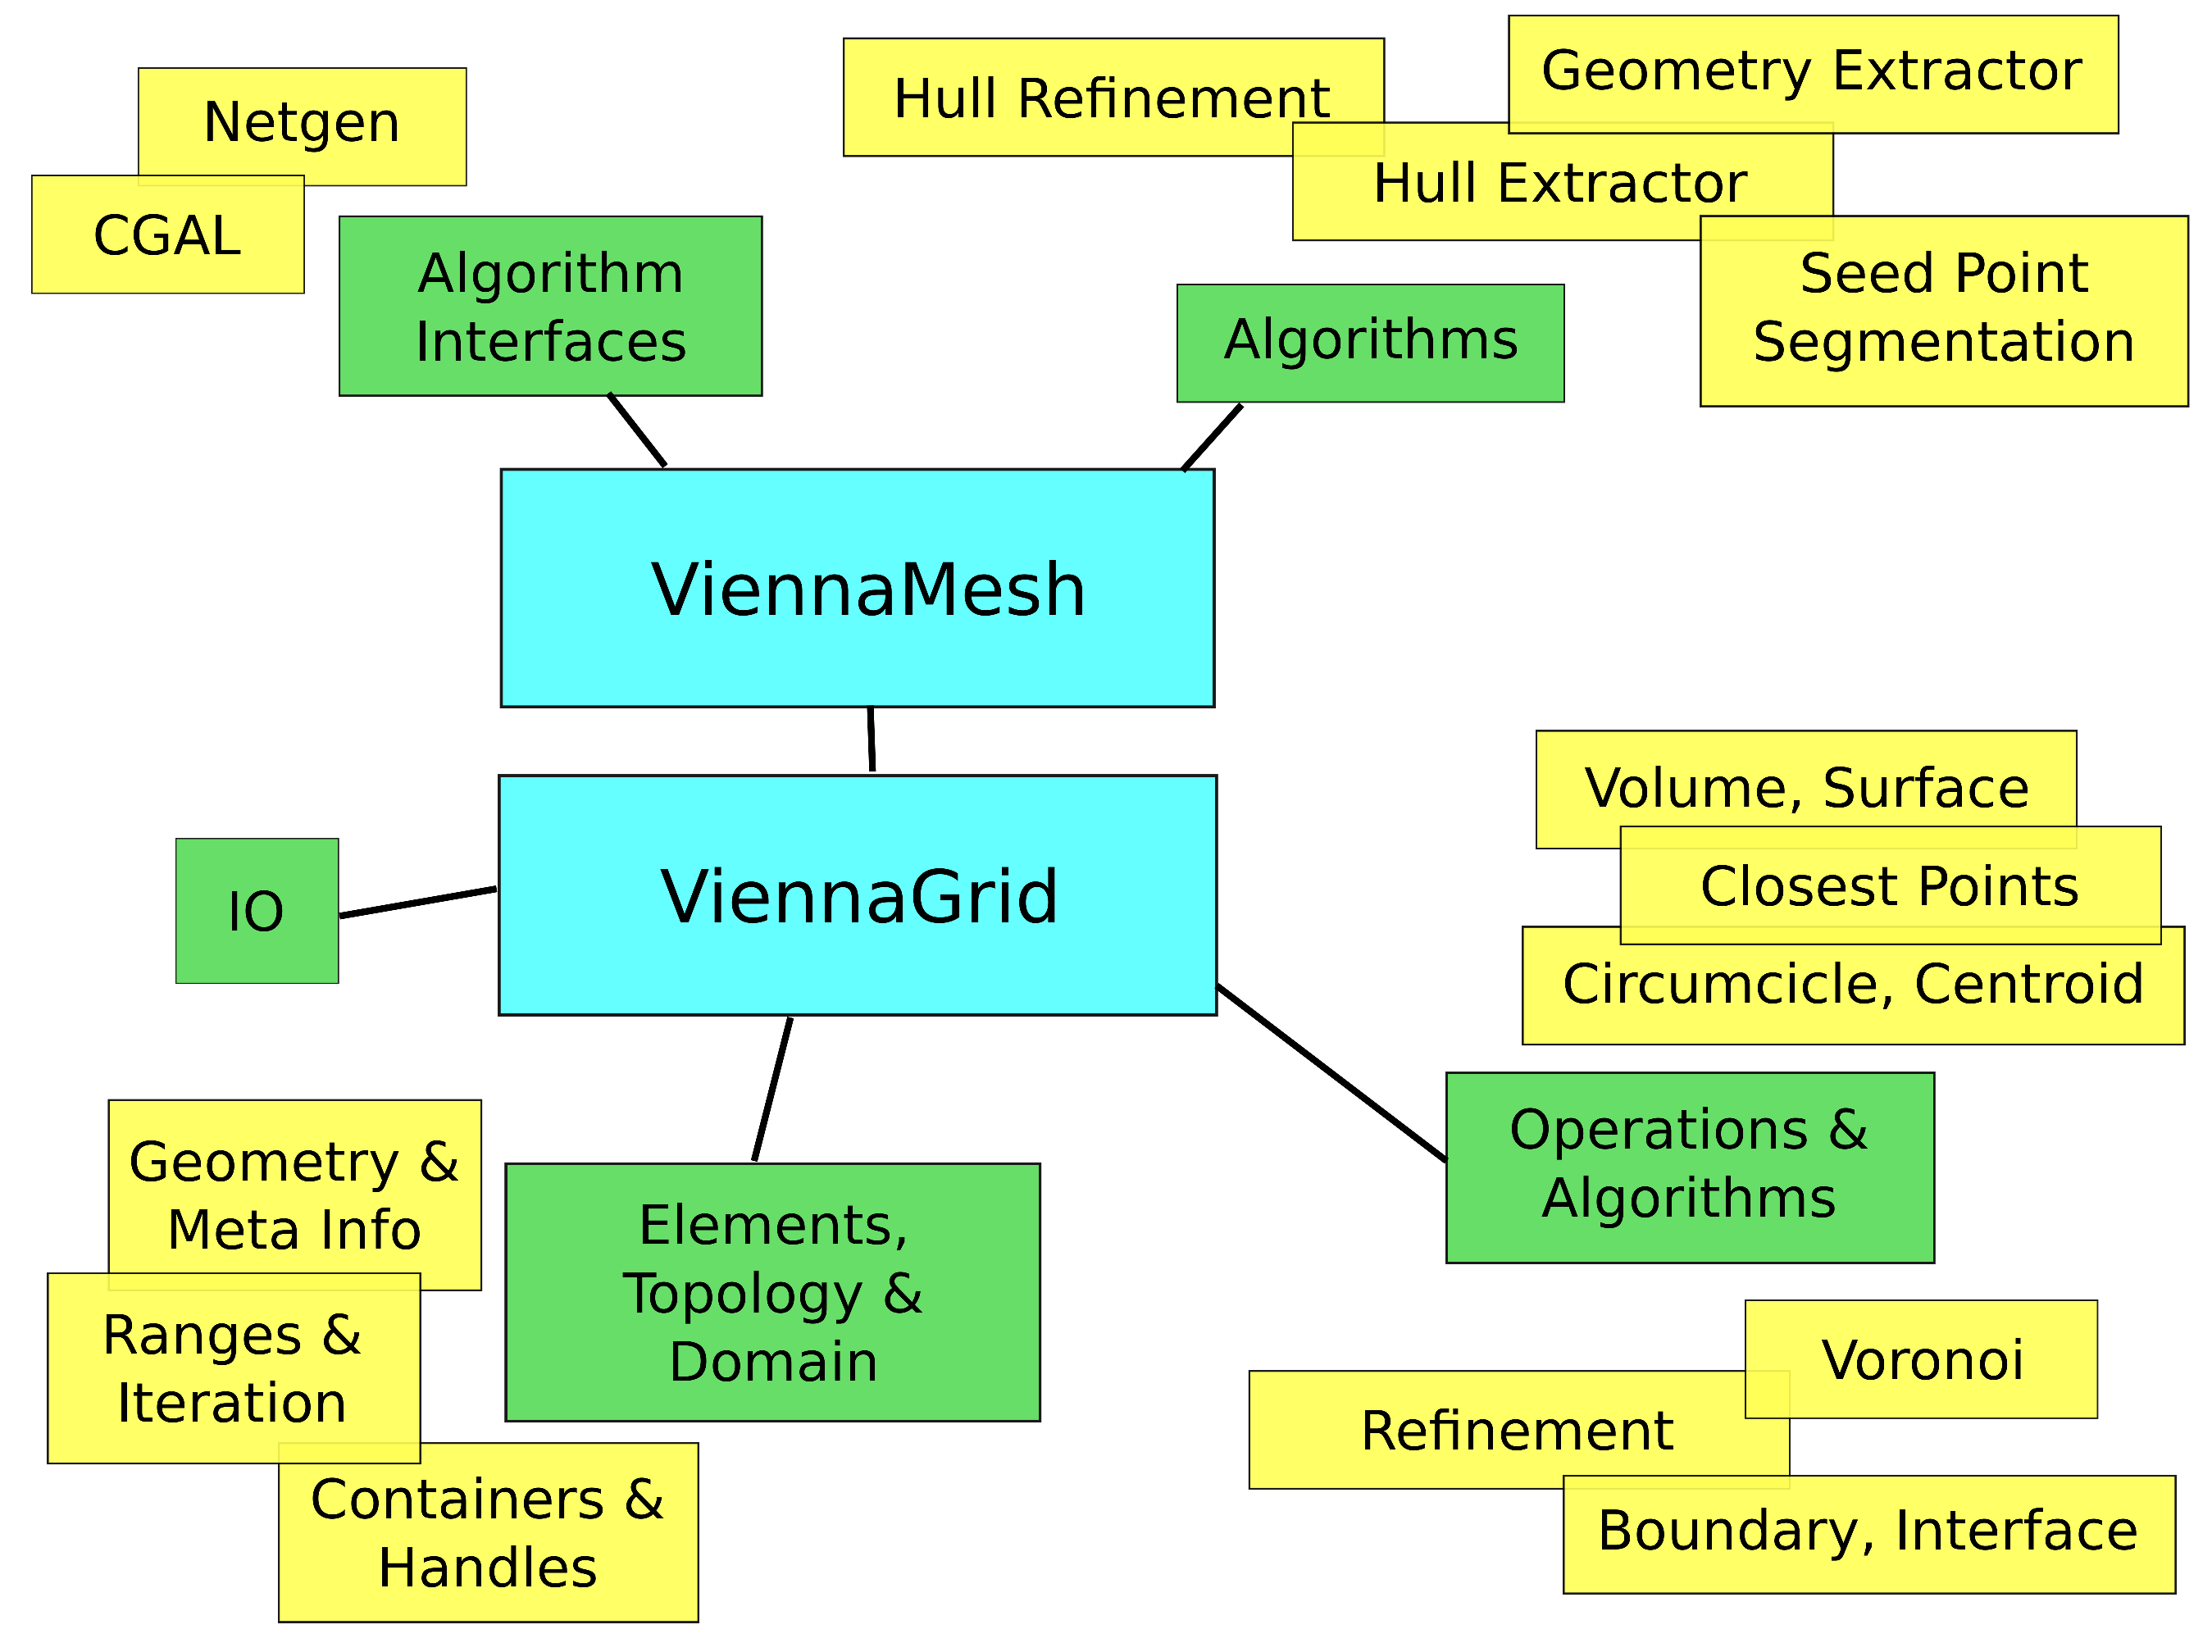
\includegraphics[scale=0.2]{figs/viennamesh_overview.eps}
    \end{figure}
  
\end{frame}



\begin{frame}[fragile]%[<+->]
  \frametitle{Framework Overview Explained}

  \begin{block}{ViennaGrid}
    \begin{itemize} \itemsep0pt \footnotesize
      \item Low level meshing data structure
      \item Central base of ViennaMesh
      \item Focus on topology, geometry as layer above topology
    \end{itemize}
  \end{block}

  \begin{block}{ViennaMesh Core}
    \begin{itemize} \itemsep0pt \footnotesize
      \item Core Meshing functionality
      \item Abstract domain concept
      \item Abstract algorithm concept
    \end{itemize}
  \end{block}
  
  \begin{block}{ViennaMesh algorithms}
    \begin{itemize} \itemsep0pt \footnotesize
      \item Interfaces to external libraries
    \end{itemize}
  \end{block}
  
\end{frame}


% ==============================================================================
\section{Data Structure - ViennaGrid}
\subsection{}


\begin{frame}[fragile]%[<+->]
  \frametitle{ViennaGrid - Types}
  
  \begin{block}{Types are queried by result\_of}
      \begin{itemize} \footnotesize
        \item Similar to C++ result\_of
        \item Tags represent element types
      \end{itemize}
  \end{block}
  
\begin{lstlisting}[linewidth=1.0 \textwidth]
typedef result_of::element<DomainType, ElementTag>
    ::type ElementType;
typedef result_of::handle<DomainType, ElementTag>
    ::type ElementHandle;

typedef result_of::vertex<DomainType>
    ::type VertexType;
typedef result_of::vertex_handle<DomainType>
    ::type VertexHandle;
\end{lstlisting}
  
\end{frame}



\begin{frame}[fragile]%[<+->]
  \frametitle{ViennaGrid - Elements}
  
  \begin{block}{Elements represent topological entities}
      \begin{itemize} \footnotesize
        \item Explicit storage of boundary elements
        \item Using handles to store boundary elements
        \item Co-Boundary and neighbour elements calculated when needed
      \end{itemize}
  \end{block}
  
  \begin{block}{Topological structures of arbitrary topological dimension}
      \begin{itemize} \footnotesize
        \item Simplices
        \item Hypercubes
      \end{itemize}
  \end{block}
  
  \begin{block}{Dynamic types supported}
      \begin{itemize} \footnotesize
        \item Polygons and PLCs
      \end{itemize}
  \end{block}
  
\end{frame}


\begin{frame}[fragile]%[<+->]
  \frametitle{ViennaGrid - Elements}
  
    \begin{figure}
        \centering
        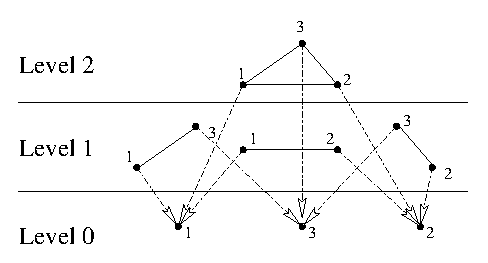
\includegraphics[scale=1.2]{figs/triangle-layers.eps}
        \caption*{Topological structure of a triangle}
    \end{figure}
  
\end{frame}



\begin{frame}[fragile]%[<+->]
  \frametitle{ViennaGrid - Topology}
  
  \begin{block}{Topological complex}
      \begin{itemize} \footnotesize
        \item Set of elements
        \item Intersection of 2 elements $\rightarrow$ empty or another element
        \item Same elements stored only once
        \item Non-conforming complexes supported (but with some restrictions)
      \end{itemize}
  \end{block}
  

  
\end{frame}



\begin{frame}[fragile]%[<+->]
  \frametitle{Example: Create Elements}
  
\begin{lstlisting}[linewidth=1.0 \textwidth]
typedef config::tetrahedral_3d_domain DomainType;

DomainType domain;

typedef result_of::element<DomainType, vertex_tag>
    ::type VertexType;
typedef result_of::element<DomainType, tetrahedron_tag>
    ::type CellType;

typedef result_of::handle<DomainType, vertex_tag>
    ::type VertexHandle;
typedef result_of::handle<DomainType, tetrahedron_tag>
    ::type CellHandle;

VertexHandle vertices[4];
for (int i = 0; i < 4; ++i)
    vertices[i]=create_element<VertexType>(domain);
    
CellHandle cell=create_element<CellType>(domain, vertices);
\end{lstlisting}
  
\end{frame}



\begin{frame}[fragile]%[<+->]
  \frametitle{Example: Create Elements}
  
\begin{lstlisting}[linewidth=1.0 \textwidth]
typedef config::tetrahedral_3d_domain DomainType;

DomainType domain;

typedef result_of::vertex_handle<DomainType>
    ::type VertexHandle;
typedef result_of::cell_handle<DomainType>
    ::type CellHandle;

VertexHandle vertices[4];
for (int i = 0; i < 4; ++i)
    vertices[i] = create_vertex(domain);
    
CellHandle cell = create_tetrahedron(domain,
    vertices[0], vertices[1], vertices[2], vertices[3]);
\end{lstlisting}
  
\end{frame}



\begin{frame}[fragile]%[<+->]
  \frametitle{Meta Information}
  
  \begin{block}{Default meta information: geometric point information}
      \begin{itemize} \footnotesize
        \item Topology only stores vertices $\rightarrow$ Geometric information needed
      \end{itemize}
  \end{block}

  \begin{block}{Storage of Geometric information}
      \begin{itemize} \footnotesize
        \item Within domain object
        \item Separate object
      \end{itemize}   
  \end{block}
  
  \begin{block}{Same interface is used}
      \begin{itemize} \footnotesize
        \item look\_up for domain separate information
        \item Usage: look\_up( domain\_or\_lunch, element )
      \end{itemize}   
  \end{block}
  
\end{frame}



\begin{frame}[fragile]%[<+->]
  \frametitle{Example: Meta Information}
  
\begin{lstlisting}[linewidth=1.0 \textwidth]
ElementType element;

deque<double> scalar_values;
map< result_of::id_type<ElementType>::type,
    string > string_values;

look_up(scalar_values, element) = 42.0;
look_up(string_values, element) = "my_element";

VertexType vertex;
std::deque<PointType> geometric_container;

point(domain, vertex) = PointType(0, 0, 1);
point(geometric_container, vertex) = PointType(0, 1, 0);
\end{lstlisting}
  
\end{frame}




\begin{frame}[fragile]%[<+->]
  \frametitle{ViennaGrid - Domain, View}
  
  \begin{block}{Domain object represents collection of elements}  
      \begin{itemize} \footnotesize
        \item Adds geometric information to topology
        \item Can be configured to work with any elements
      \end{itemize}
  \end{block}

  \begin{block}{View represents subsets of the domain}
      \begin{itemize} \footnotesize
        \item Uses handle to store references
        \item Can be used to define segments
      \end{itemize}   
  \end{block}
  
\end{frame}




\begin{frame}[fragile]%[<+->]
  \frametitle{Example: Geometric Information}
  
\begin{lstlisting}[linewidth=1.0 \textwidth]
typedef config::tetrahedral_3d_domain DomainType;
typedef result_of::point_type<DomainType>::type PointType;

DomainType domain;

typedef result_of::vertex_handle<DomainType>
    ::type VertexHandle;
typedef result_of::cell_handle<DomainType>
    ::type CellHandle;

VertexHandle vertices[4];
for (int i = 0; i < 4; ++i)
{
  vertices[i] = create_vertex(domain);
  point( domain, vertices[i] ) = PointType(i, i*i, i*i*i);
}
    
CellHandle cell = create_tetrahedron(domain,
    vertices[0], vertices[1], vertices[2], vertices[3]);
\end{lstlisting}
  
\end{frame}



\begin{frame}[fragile]%[<+->]
  \frametitle{Example: Create View}
  
\begin{lstlisting}[linewidth=1.0 \textwidth]
typedef config::tetrahedral_3d_domain DomainType;
typedef config::tetrahedral_3d_view ViewType;

DomainType domain;
ViewType view = create_view( domain );

typedef result_of::vertex_handle<DomainType>
    ::type VertexHandle;
typedef result_of::cell_handle<DomainType>
    ::type CellHandle;

VertexHandle vertices[4];
for (int i = 0; i < 4; ++i)
    vertices[i] = create_vertex(domain);
    
CellHandle cell = create_tetrahedron(view,
    vertices[0], vertices[1], vertices[2], vertices[3]);
\end{lstlisting}
  
\end{frame}



\begin{frame}[fragile]%[<+->]
  \frametitle{ViennaMesh - Segment Support}
  
  \begin{minipage}[t]{0.48\linewidth}
    \begin{block}{Support for segments}
        \begin{itemize} \footnotesize
            \item Subsets of the mesh
            \item Preserve interfaces through\\meshing process
        \end{itemize}
    \end{block}
  \end{minipage}
  \begin{minipage}[t]{0.48\linewidth}
    \begin{figure}
            \centering
            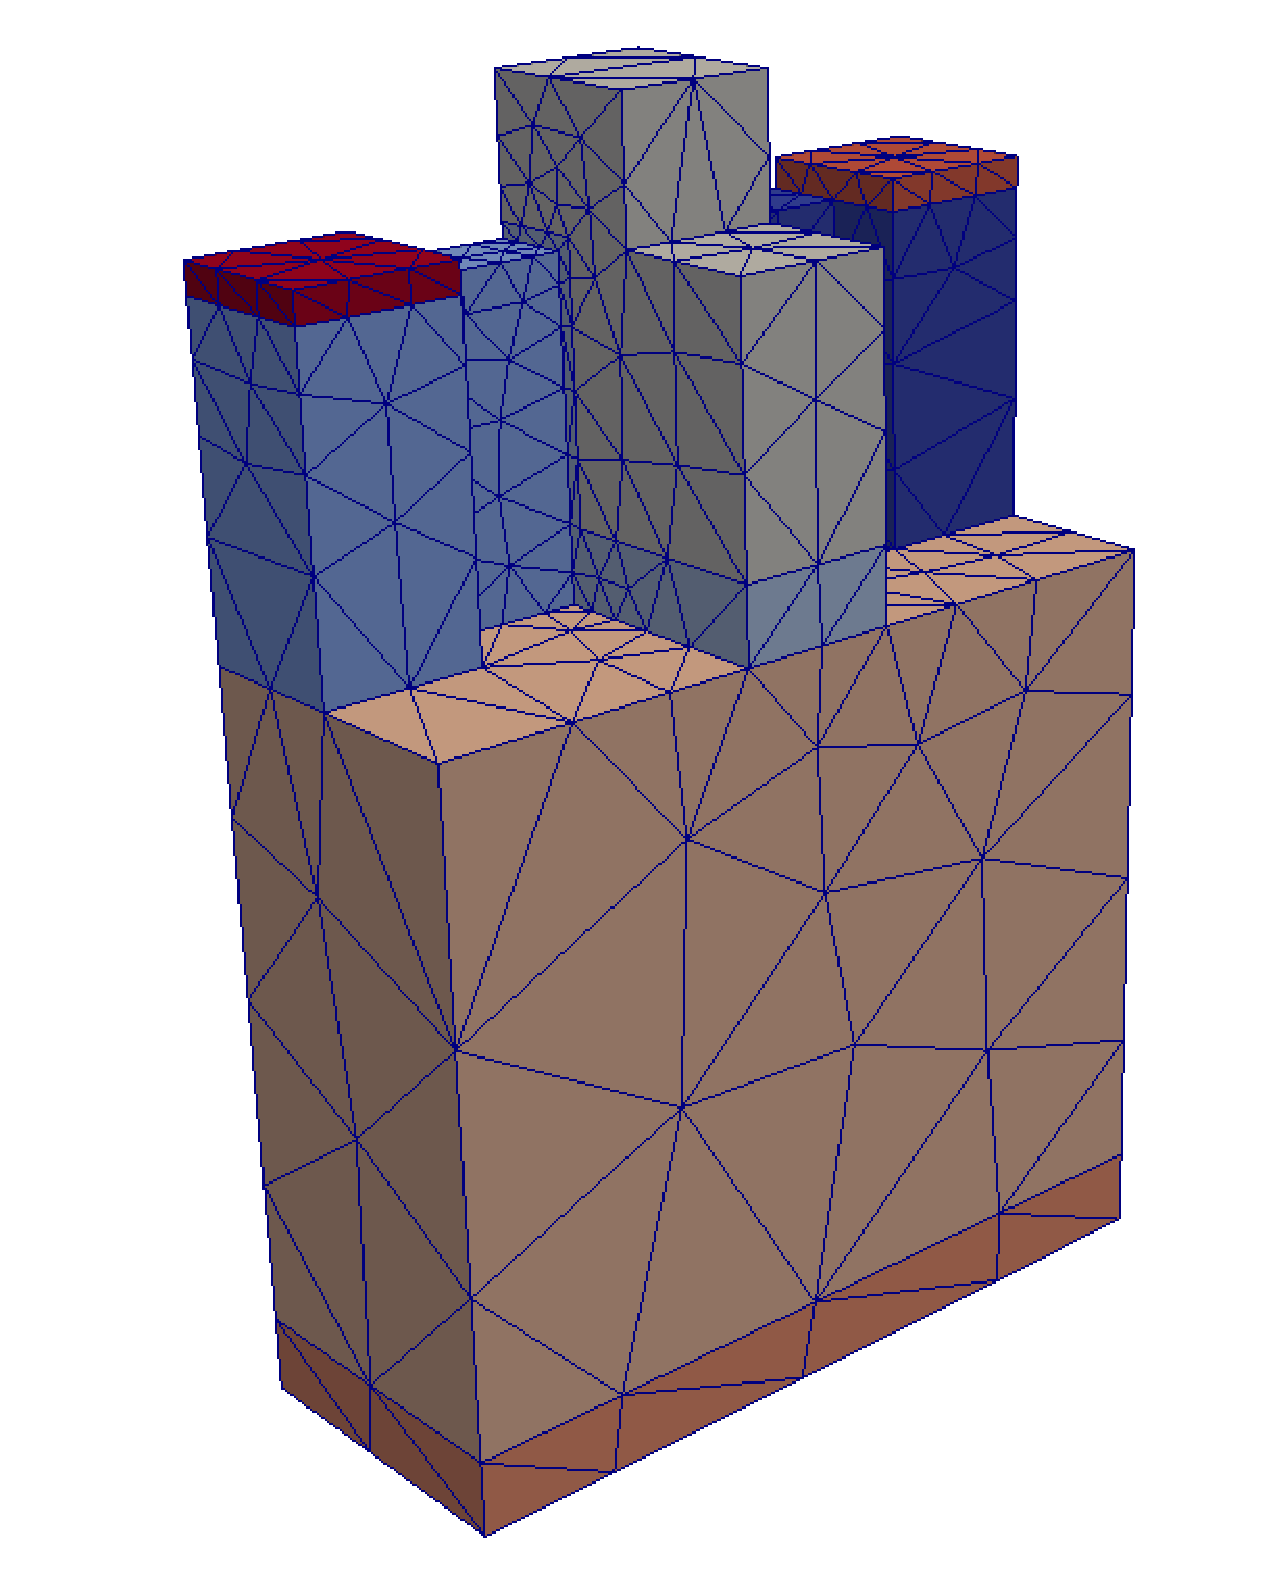
\includegraphics[scale=0.15]{figs/segments.eps}
    \end{figure}
  \end{minipage}

\end{frame}



\begin{frame}[fragile]%[<+->]
  \frametitle{ViennaGrid - Segmentation}
  
  \begin{block}{Segmentations with Views}  
      \begin{itemize} \footnotesize
        \item Using Views for segmentation
        \item One per segment
        \item Using seed points
      \end{itemize}
  \end{block}

  \begin{block}{Segmentation object}
      \begin{itemize} \footnotesize
        \item Stores segment information per element
        \item Trivial segment information: segment id
        \item Segment information for hull domain: with orientation
      \end{itemize}   
  \end{block}
  
\end{frame}



\begin{frame}[fragile]%[<+->]
  \frametitle{Example: Segmentation}
  
\begin{lstlisting}[linewidth=1.0 \textwidth]
typedef config::triangular_3d_domain DomainType;
typedef config::triangular_3d_segmentation SegmentationType;

DomainType domain;
SegmentationType segmentation =
    viennagrid::create_segmentation(domain);

TriangleType triangle;

segmentation.segment_info(triangle).
    positive_orientation_segment_id = segment_id_0;
segmentation.segment_info(triangle).
    negative_orientation_segment_id = segment_id_1;
\end{lstlisting}
  
\end{frame}



\begin{frame}[fragile]%[<+->]
  \frametitle{ViennaGrid - Containers, Handles and Ranges}
  
  \begin{block}{Generic low level storage system}
      \begin{itemize} \footnotesize
        \item Container and handle types are configurable
        \item Default container: std::deque
        \item Default handle: pointer to element
      \end{itemize}   
  \end{block}

  \begin{block}{Range defines a set or subset of elements}
      \begin{itemize} \footnotesize
        \item Needed for iteration
      \end{itemize}   
  \end{block}
  
\end{frame}



\begin{frame}[fragile]%[<+->]
  \frametitle{ViennaGrid - Iteration}
  
  \begin{block}{Iteration is type-independent}
      \begin{itemize} \footnotesize
        \item Easy access of associated elements
        \item Same source code for different types
      \end{itemize}
  \end{block}
  
  \begin{block}{Element Iteration}  
      \begin{itemize} \footnotesize
        \item Iterating over elements of a domain or view
      \end{itemize}
  \end{block}
  
\end{frame}



\begin{frame}[fragile]%[<+->]
  \frametitle{ViennaGrid - Iteration}
  
  \begin{block}{Boundary Element Iteration}
      \begin{itemize} \footnotesize
        \item Iterating over boundary elements of an element
        \item Same as element iteration
      \end{itemize}   
  \end{block}
  
  \begin{block}{Co-Boundary Element Iteration}
      \begin{itemize} \footnotesize
        \item Iterating over co-boundary elements of an element
        \item Scope domain or view is needed
      \end{itemize}   
  \end{block}
  
%   \begin{block}{Neighbor Element Iteration}
%       \begin{itemize} \footnotesize
%         \item Iterating over neighbour elements of an element
%         \item Scope domain or view is needed
%       \end{itemize}   
%   \end{block}
  
\end{frame}



\begin{frame}[fragile]%[<+->]
  \frametitle{Example: Iteration Domain/View}
  
\begin{lstlisting}[linewidth=1.0 \textwidth]
DomainType domain;

typedef result_of::element_range<DomainType, vertex_tag>
    ::type VertexRangeType;
typedef result_of::iterator<VertexRangeType>
    ::type VertexRangeIterator;

VertexRangeType vertices = elements( domain );
for (VertexRangeIterator it = vertices.begin();
     it != vertices.end(); ++it)
{
    cout << point(domain, *it) << endl;
}
\end{lstlisting}
  
\end{frame}



\begin{frame}[fragile]%[<+->]
  \frametitle{Example: Boundary Element Iteration}
  
\begin{lstlisting}[linewidth=1.0 \textwidth]
ElementType element;

typedef result_of::element_range<ElementType, vertex_tag>
    ::type VertexOnElementRangeType;
typedef result_of::iterator<VertexOnElementRangeType>
    ::type VertexOnElementRangeIterator;

VertexOnElementRangeType vertices = elements( element );
for (VertexOnElementRangeIterator it = vertices.begin();
    it != vertices.end(); ++it)
{
    cout << point(domain, *it) << endl;
}
\end{lstlisting}
  
\end{frame}



\begin{frame}[fragile]%[<+->]
  \frametitle{Example: Co-Boundary Element Iteration}
  
\begin{lstlisting}[linewidth=1.0 \textwidth]
DomainType domain;
VertexType vertex;

typedef result_of::coboundary_range<DomainType, triangle_tag>
    ::type TrianglesOfVertexRangeType;
typedef result_of::iterator<TrianglesOfVertexRangeType>
    ::type TrianglesOfVertexRangeIterator;

TrianglesOfVertexRangeType triangles =
    coboundary_elements( domain, vertex );
for (TrianglesOfVertexRangeIterator it = triangles.begin();
    it != triangles.end(); ++it)
{
    // do something with triangle *it
}
\end{lstlisting}
  
\end{frame}



% \begin{frame}[fragile]%[<+->]
%   \frametitle{Example: Neighbour Element Iteration}
%   
% \begin{lstlisting}[linewidth=1.0 \textwidth]
% DomainType domain;
% TriangleHandleType triangle_handle;
% 
% typedef result_of::neighbour_range<DomainType,
%     triangle_tag>::type NeighbourTriangleRangeType;
% typedef result_of::iterator<
%     NeighbourTriangleRangeType>::type NeighbourTriangleRangeIterator;
% 
% NeighbourTriangleRangeType triangles = neighbour_elements<vertex_tag>( domain, triangle_handle );
% for (NeighbourTriangleRangeIterator it = triangles.begin(); it != triangles.end(); ++it)
% {
%     // do something with triangle *it
% }
% \end{lstlisting}
%   
% \end{frame}




\begin{frame}[fragile]%[<+->]
  \frametitle{IO}
  
  \begin{block}{Supported file reader}
      \begin{itemize} \footnotesize
        \item VTK
        \item Netgen
        \item Tetgen poly (PLC)
      \end{itemize}
  \end{block}

  \begin{block}{Supported file writer}
      \begin{itemize} \footnotesize
        \item VTK
        \item OpenDX
      \end{itemize}   
  \end{block}
  
  \begin{block}{VTK reader and writer supports meta data}
      \begin{itemize} \footnotesize
        \item support for vertices and cells
      \end{itemize}
  \end{block}
  
\end{frame}



% ==============================================================================
\section{ViennaGrid - Algorithms}
\subsection{}

\begin{frame}[fragile]%[<+->]
  \frametitle{Overview ViennaGrid Operations and Algorithms}
  
  \begin{block}{Element based operations and algorithms}
      \begin{itemize} \footnotesize
        \item Use only local element information
        \item e.g. volume
      \end{itemize}
  \end{block}

  \begin{block}{Domain based algorithms}
      \begin{itemize} \footnotesize
        \item Requires domain/view context
        \item e.g. refine
      \end{itemize}   
  \end{block}

\end{frame}


% \begin{frame}[fragile]%[<+->]
%   \frametitle{Element based algorithms}
%   
%   \begin{block}{Volume}
%       \begin{itemize} \footnotesize
%         \item Calculates the volume of a specific element
%         \item Volume of domain/view is also implemented
%       \end{itemize}
%   \end{block}
% 
%   \begin{block}{Surface}
%       \begin{itemize} \footnotesize
%         \item Calculates the surface of a specific element
%         \item Implemented by using volume on specified boundary elements
%         \item Surface of domain/view is implemented using is\_boundary
%       \end{itemize}   
%   \end{block}
% 
% \end{frame}


\begin{frame}[fragile]%[<+->]
  \frametitle{Element based operations and algorithms}
  
  \begin{block}{More element operations and algorithms available}
      \begin{itemize} \footnotesize
        \item Volume
        \item Surface
        \item Inner product
        \item Norm
        \item Cross product
        \item Centroid
        \item Circumcircle
        \item Closest points
      \end{itemize}
  \end{block}

\end{frame}




\begin{frame}[fragile]%[<+->]
  \frametitle{Example: Volume data transfer}

  \begin{block}{Transfer data from triangle to vertex}
    \begin{itemize} \footnotesize
      \item value weighted with triangle volume
    \end{itemize}
  \end{block}
  
\begin{lstlisting}[linewidth=1.0 \textwidth]
for (auto v : viennagrid::vertices( domain ) )
{
  numeric_type weighted_value = 0, total_volume = 0;

  for ( auto t : viennagrid::triangles(domain, v) )
  {
    numeric_type current_volume = volume( domain, t );
    total_volume += current_volume;
    weighted_value += current_volume * value(t);
  }

  value(v) = weighted_value / total_volume;
}
\end{lstlisting}
\end{frame}



\begin{frame}[fragile]%[<+->]
  \frametitle{Example: Volume data transfer}

  \begin{block}{Type independent implementation}
    \begin{itemize} \footnotesize
      \item to\_tag and from\_tag specify the types
    \end{itemize}
  \end{block}
  
\begin{lstlisting}[linewidth=1.0 \textwidth]
|\color{blue}for (auto v : viennagrid::elements<to\_tag>( domain ) )|
{
  numeric_type weighted_value = 0, total_volume = 0;

  |\color{blue}for ( auto t : viennagrid::coboundary\_elements<from\_tag>(domain, v) )|
  {
    numeric_type current_volume = volume( domain, t );
    total_volume += current_volume;
    weighted_value += current_volume * value(t);
  }

  value(v) = weighted_value / total_volume;
}
\end{lstlisting}
\end{frame}




\begin{frame}[fragile]%[<+->]
  \frametitle{Domain based algorithms}
  
  \begin{block}{Boundary}
      \begin{itemize} \footnotesize
        \item Determines if the current element is a boundary element
        \item Requires domain/view context
      \end{itemize}
  \end{block}
  
  \begin{block}{Refine}
      \begin{itemize} \footnotesize
        \item Refines previously marked cells
      \end{itemize}
  \end{block}
  
  \begin{block}{Voronoi}
      \begin{itemize} \footnotesize
        \item Calculates the voronoi information of a domain/view
      \end{itemize}
  \end{block}

\end{frame}



\begin{frame}[fragile]%[<+->]
  \frametitle{Example: Refinement}

    \begin{figure}
        \centering
        \begin{subfigure}[b]{60mm}
            \centering
            \includegraphics[scale=0.13]{figs/sshape_3d_1.eps}
            \caption*{Before Refinement}
        \end{subfigure}%
    \end{figure}
  
\end{frame}



\begin{frame}[fragile]%[<+->]
  \frametitle{Example: Refinement}

    \begin{figure}
        \centering
        \begin{subfigure}[b]{60mm}
            \centering
            \includegraphics[scale=0.13]{figs/sshape_3d_2.eps}
            \caption*{After Refinement}
        \end{subfigure}%
    \end{figure}
  
\end{frame}



\begin{frame}[fragile]%[<+->]
  \frametitle{Example: Refinement}
  
\begin{lstlisting}[linewidth=1.0 \textwidth]
for (auto element : cells(domain) )
{
  if (to_refine(element))
    tag_to_refine(element);
}

refine(domain, segments,
       result_domain, result_segments,
       local_refinement_tag() );
\end{lstlisting}
  
\end{frame}



% ==============================================================================
\section{ViennaMesh - Algorithms}
\subsection{}

\begin{frame}[fragile]%[<+->]
  \frametitle{ViennaMesh Domain Concept}
  
  \begin{block}{ViennaMesh aims to support external libraries}
      \begin{itemize} \footnotesize
        \item Interfaces have to be provided
      \end{itemize}
  \end{block}
  
  \begin{minipage}[t]{0.65\linewidth}
    \begin{block}{Each external library comes with its own data structure}
    \end{block}
  \end{minipage}
  \begin{minipage}[t]{0.30\linewidth}
    \begin{figure}
        \centering
        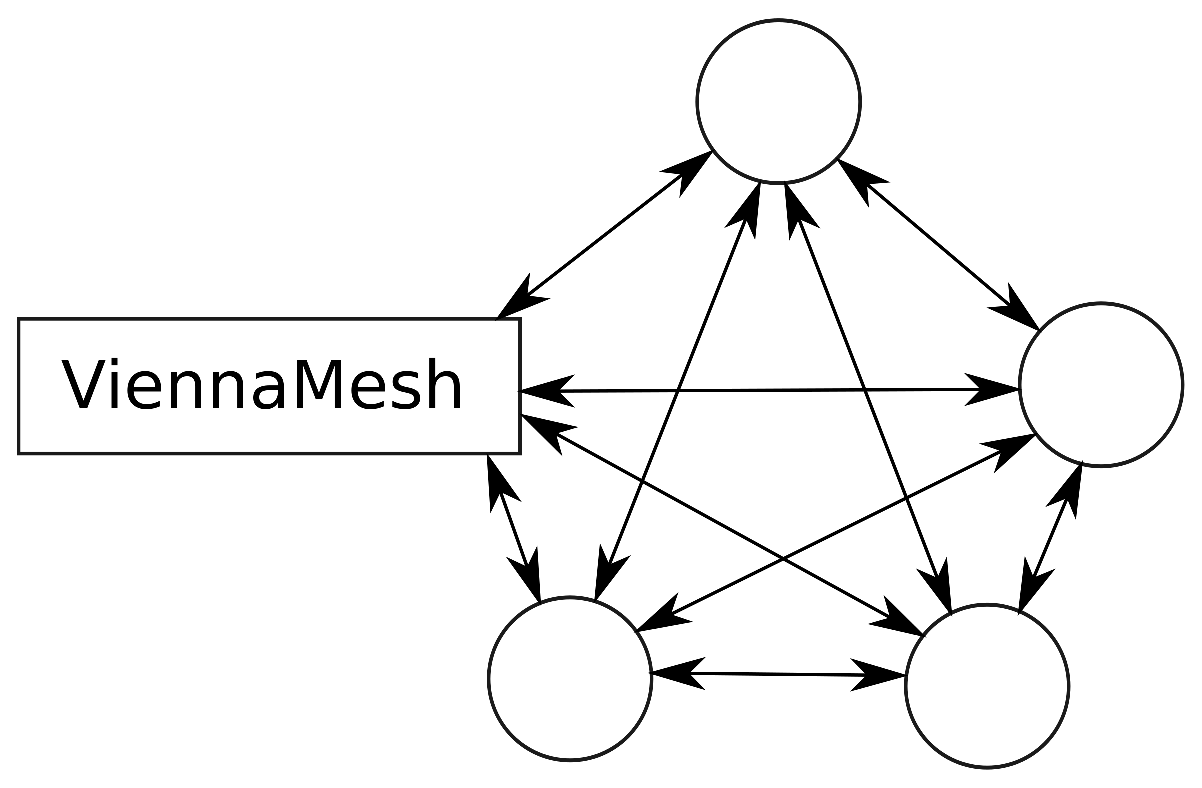
\includegraphics[scale=0.18]{figs/conversion.eps}
    \end{figure}
  \end{minipage}
  
\end{frame}



\begin{frame}[fragile]%[<+->]
  \frametitle{ViennaMesh Domain Concept}
  
  \begin{block}{ViennaMesh aims to support external libraries}
      \begin{itemize} \footnotesize
        \item Interfaces have to be provided
      \end{itemize}
  \end{block}
  
  \begin{minipage}[t]{0.65\linewidth}
    \begin{block}{Each external library comes with its own data structure}
      \begin{itemize} \footnotesize
        \item Conversions to and from ViennaGrid required
        \item Other conversions optional
      \end{itemize}
    \end{block}
  \end{minipage}
  \begin{minipage}[t]{0.30\linewidth}
    \begin{figure}
            \centering
            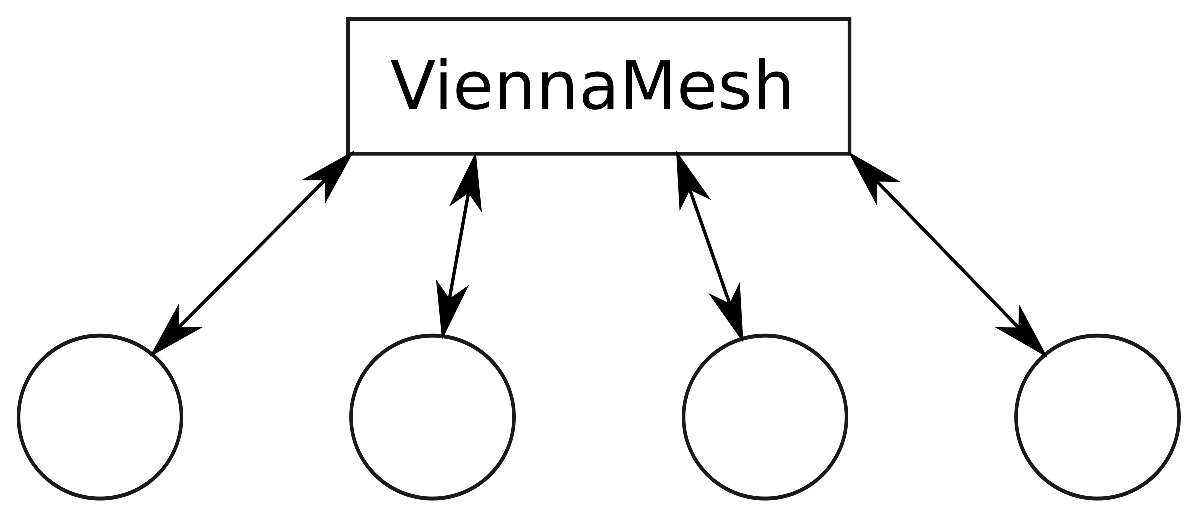
\includegraphics[scale=0.18]{figs/conversion_viennamesh.eps}
    \end{figure}
  \end{minipage}
  
\end{frame}



\begin{frame}[fragile]%[<+->]
  \frametitle{ViennaMesh Algorithm Concept}
  
  \begin{block}{ViennaMesh provides an uniform interface for complex algorithms}
      \begin{itemize} \footnotesize
        \item Query algorithm information and settings object
      \end{itemize}
  \end{block}
  
  \begin{block}{Execution of algorithm is generic interface}
      \begin{itemize} \footnotesize
        \item viennamesh::run\_algo$<$algorithm\_tag$>$( source, destination, settings )
        \item If required, source and destination is converted implicitly
      \end{itemize}
  \end{block}
  
  \begin{block}{Returns information of algorithm execution}
      \begin{itemize} \footnotesize
        \item Execute time
        \item Success state
        \item Errors, warnings and informations
      \end{itemize}
  \end{block}

\end{frame}


\begin{frame}[fragile]%[<+->]
  \frametitle{ViennaMesh Algorithms}
  
  \begin{block}{Internal algorithms in ViennaMesh}
      \begin{itemize} \footnotesize
        \item Extract Hull
        \item Extract PLC Geometry
        \item Seed point segment marking of hull meshes
        \item Multi-segment hull refinement
        \item Mesh doctor: 3D triangular hull
      \end{itemize}
  \end{block}
  
  \begin{block}{External algorithms with ViennaMesh interface}
      \begin{itemize} \footnotesize
        \item Netgen: triangular hull $\rightarrow$ tetrahedral volume
        \item CGAL: PLC $\rightarrow$ triangular hull (2D and 3D)
        \item CGAL: triangular hull $\rightarrow$ tetrahedral volume
      \end{itemize}
  \end{block}

\end{frame}



\begin{frame}[fragile]%[<+->]
  \frametitle{ViennaMesh Algorithms}

  \begin{block}{External and internal algorithms share common interface}
      \begin{itemize} \footnotesize
        \item data structure conversion if needed
      \end{itemize}
  \end{block}

\begin{lstlisting}[linewidth=1.0\textwidth]
InputDomainType  input_domain;
OutputDomainType output_domain;
viennamesh::result_of::settings<algorithm_tag>::type
                settings;
                
settings.cell_size = 1.0;

viennamesh::run_algo< algorithm_tag >(
    |\color{blue}input\_domain|,
    |\color{blue}output\_domain|,
    settings);
\end{lstlisting}

\end{frame}



\begin{frame}[fragile]%[<+->]
  \frametitle{ViennaMesh Algorithms}

  \begin{block}{External and internal algorithms share common interface}
      \begin{itemize} \footnotesize
        \item Easy exchangeability of algorithms
      \end{itemize}
  \end{block}

\begin{lstlisting}[linewidth=1.0\textwidth]
InputDomainType  input_domain;
OutputDomainType output_domain;
viennamesh::result_of::settings< |\color{blue}algorithm\_tag| >::type
                settings;

settings.cell_size = 1.0;
                
viennamesh::run_algo< |\color{blue}algorithm\_tag| >(
    input_domain,
    output_domain,
    settings);
\end{lstlisting}

\end{frame}




\begin{frame}[fragile]%[<+->]
  \frametitle{ViennaMesh Examples}

  \centering
  Time for some detailed source code! :-)

\end{frame}



% \begin{frame}[fragile]%[<+->]
%   \frametitle{Example: Boost.Accumulators}
%   
% \begin{lstlisting}[linewidth=1.0 \textwidth]
% result_of::element_range<
%   DomainType, tetrahedron_tag>::type
%   ElementRange;
%        
% BoostAccumulatorType acc;       
%        
% ElementRange tetrahedrons = elements(domain);
% 
% std::for_each( domain.begin(), domain.end(),
%   [&domain, &acc](ElementRange::value_type & element)
%   { acc(aspect_ratio(domain, element)); } );
% \end{lstlisting}
%   
% \end{frame}


% \begin{frame}[fragile]%[<+->]
%   \frametitle{Example: CGAL Tetrahedral Meshing}
%   
% \begin{lstlisting}[linewidth=1.0 \textwidth]
% config::plc_3d_domain plc_domain;
% result_of::settings<cgal_plc_3d_mesher_tag>::type
%     plc_settings;
% 
% config::triangular_3d_domain triangle_domain;
% run_algo< cgal_plc_3d_mesher_tag >( plc_domain,
%     triangle_domain,
%     plc_settings );
% 
% result_of::settings<cgal_delaunay_tetrahedron_tag>::type
%     tetrahedron_settings;
% 
% deltet_settings.cell_size = 2.0;
% 
% config::tetrahedral_3d_domain tetrahedron_domain;
% run_algo<cgal_delaunay_tetrahedron_tag>(triangle_domain,
%     tetrahedron_domain,
%     tetrahedron_settings);
% \end{lstlisting}
%   
% \end{frame}


% \begin{frame}[fragile]%[<+->]
%   \frametitle{Example: Hull extractor}
%   
% \begin{lstlisting}[linewidth=1.0 \textwidth]
% TetrahedronDoimanType tetrahedron_domain;
% deque<TetrahedronViewType> tetrahedron_segments;
% 
% TriangleDomainType triangle_domain;
% deque<TriangleViewType> triangle_segments;
% 
% result_of::settings<extract_hull_tag>::type
%     extract_hull_settings;
% 
% run_algo<extract_hull_tag>(
%   tetrahedron_domain, tetrahedron_segments,
%   triangle_domain, triangle_segments,
%   extract_hull_settings );
% \end{lstlisting}
%   
% \end{frame}


% ==============================================================================
\section{Conclusion}
\subsection{}

\begin{frame}[fragile]%[<+->]
  \frametitle{Conclusion}
  
  \begin{block}{Flexibility}
    \begin{itemize} \footnotesize
      \item Abstract concepts $\rightarrow$ Write your code only once
      \item Common interface $\rightarrow$ Easily change meshing kernel
      \item High configurability $\rightarrow$ Use arbitrary topological structures
      \item High extensibility $\rightarrow$ Write your own meshing algorithm
    \end{itemize}
  \end{block}
  
  \begin{block}{Status}
  \begin{itemize} \footnotesize
    \item Development release available at sourceforge
    \item http://viennamesh.sourceforge.net
  \end{itemize}
  \end{block}
\end{frame}

% ==============================================================================




\end{document}





